\documentclass[a0paper, portrait]{baposter}
\usepackage{graphicx}
\usepackage[english]{babel}
\usepackage{calligra}
%\usepackage[usenames]{color}
%\usepackage[usenames,dvipsnames]{xcolor}

\definecolor{headercol}{RGB}{36,180,242}

\begin{document}
\begin{poster}{
    % Poster Environment Options
    grid=false,
    columns=3,
    colspacing=0.75cm, % subject to change
    headerheight=0.1\textheight,
    background=plain,
    bgColorOne=white,
    eyecatcher=true,
    %Postbox environment options
    borderColor=black,
    headerColorOne=headercol,
    headerColorTwo=headercol,
    textborder = roundedsmall,
    headerborder=closed,
    headershape=roundedleft,
    headershade=plain,
    boxshade=none,
    linewidth=0.20cm
}
  % Eye Catch
  { 
\includegraphics[height=0.1\textheight]{ciidit.png} }
  % Title
  {\bf\textsc{Generation of Topic Tag Clouds}} 
  % Author
  {
    Jes\'us Antonio Soto Vel\'azquez 
  }
  % Logo
  {
    
\includegraphics[height=8.0em]{uanl.png}
  }

  %%
  %% Poster Content
  %%

  % BOX1
  \headerbox{Intro}{name=intro, column=0, row=0} {
    Tag clouds aid users to recognize at a first glance what a group of various documents is about by displaying the most relevant words or topics.
    \newline
%    \begin{figure*}[ht!]
%      \caption{Magia}
%      \label{figure:01}
%      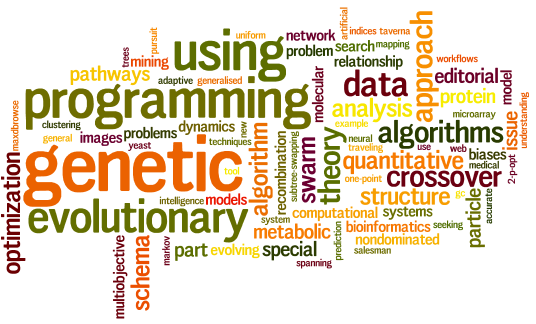
\includegraphics[height=0.1\textheight]{wordle2.png}
%    \end{figure*}

    %\centerline{\in\caption{Fig. 1 Initial tag cloud using Wordle}
    %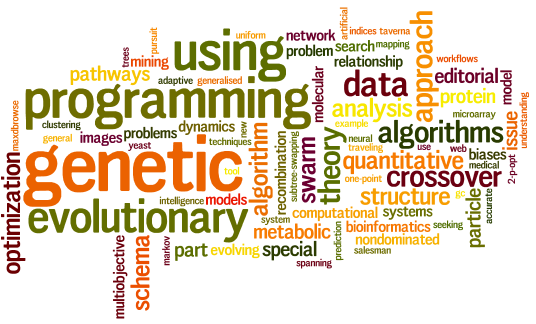
\includegraphics[height=0.1\textheight]{wordle2.png}
    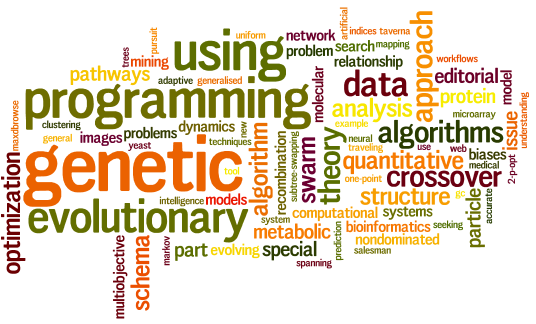
\includegraphics[width=\linewidth]{wordle2.png}
    \newline
    The {\bf objective} is to deploy a web platform which generates tag clouds with meaningful information extracted from a collection of documents. This work focuses on such an insightful {\em visualization} of the topics in the documents. %while also considering possible interaction with the tag cloud to retrieve more information. % reword plz
  }

  %BOX2
  \headerbox{Tackling the problem}{name=tech, column=0, below=intro} {
    Several aspects were taken into account when choosing the right information to put in the tag cloud, such as: \newline
    \begin{description}
    \item[Stopword filtering] Unimportant words in the given context were discaraded. Resolved with {\em String matching algorithms}.
    \item[Word stemming] Words with the same root were grouped together. Resolved with the {\em Snowball library}.
    \item[Language detection] Articles in other languages were to be excluded from the tag clouds. Resolved with the {\em language-detection library}.
    \item[The tag cloud] Manage structure and appearance of a tag cloud. Resolved with the {\em OpenCloud java library}.
    \item[Portability] As the intention was to reach as many users as possible, a web environment was chosen. Technologies used:{\em HTML5, CSS, Javascript, Servlets}
    \end{description}
  }
  %BOX3
  \headerbox{Initial solution}{name=initial, column=0, below=tech} {
    The initial solution made use of OpenCloud, a library in Java that facilitates the creation of tag clouds for the web. Using HTML and CSS, the tag cloud was given the desired styling and presentation.
    
    %\caption{Fig. 2 Tag cloud with specialized stopword filtering}
    %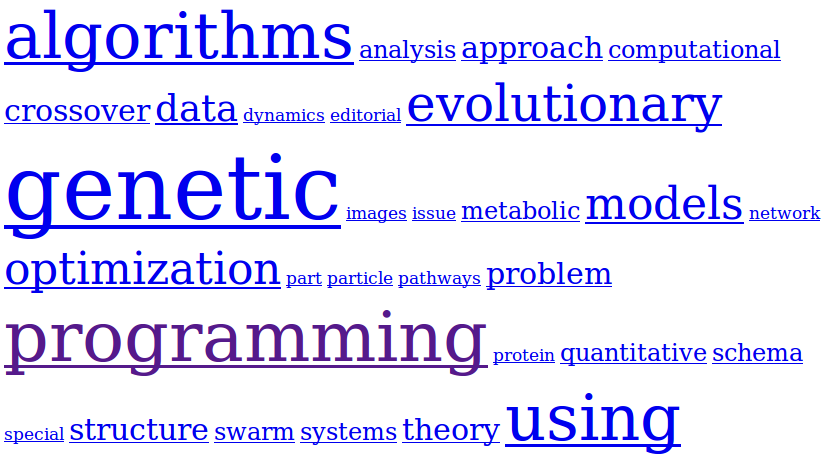
\includegraphics[height=0.1\textheight]{initial.png}
    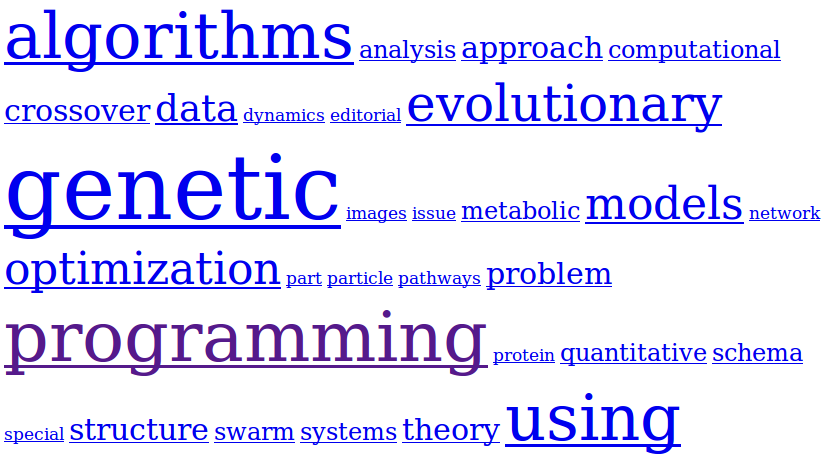
\includegraphics[width=\linewidth]{initial.png}
  }

  %BOX4
  \headerbox{Semantic approach}{name=semantic, column=1} {
    Rather than focusing on the artistic side of tag clouds, like most tag cloud tools do, an approach on semantic similarity between topics was taken. As such, the position of each topic is determined by the semantic similarity of itself and its surroundings.
    \newline
    %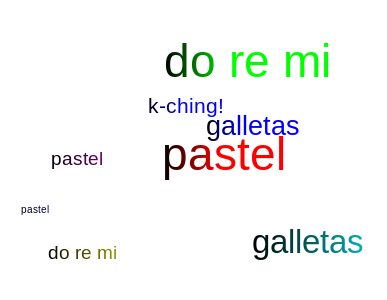
\includegraphics[height=0.1\textheight]{newcloud.png}
    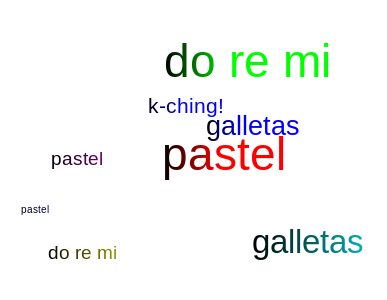
\includegraphics[width=\linewidth]{newcloud.png}
  }

  %BOX5
  \headerbox{Interacting with users}{name=interact, below=semantic, column=1} {
    The first step to allow interaction with the tag cloud was through the functionality of clicking a word in the tag cloud, and firing an event for that particular word. This was done by looking for a match of the cursor's coordinates and all of the words' coordinates.  
  }

  %BOX5.5
  \headerbox{Topic activity}{name=gradient, below=interact, column=1} {
    It might be of interest knowing how active or inactive the topics have been throughout the years. For such cases, a two-color gradient is used to represent how active each of the topics have been, or to know if its use has declined after some time. The brighter the color, the more active it is. % Last line seems kinda obvious.

    % Fig. 4 Coloring in the tag cloud
    %\includegraphics[height=0.1\textheight]{gradients.png}
    \includegraphics[width=\linewidth]{gradients.png}

  }

  %BOX6
  \headerbox{Indexing documents}{name=index, column=2} {
    In order to quickly search through the documents by typing a keyword, a structure known as an index was used. The tool used to index the groups of articles, Solr, provides a simple interface between the data stored and the means of returning the desired information in a web environment. The data is stored and structured as XML. % May delete last sentence.

    % Is a fig. suitable here?
  }
  
  %BOX7
  \headerbox{Future Work}{name=future, below=index, column=2} {
    Although the project focused on the many components involved, there is much work to be done to integrate these parts into a system for use in the web. Key points to advance development are:
    \begin{itemize}
      \item Data retrieval from tag cloud. Through user interaction, more information about the selected topic can be obtained, such as researchers involved.
      \item Given a document from the index in XML, a tag cloud should be generated.
      % \item I feel I'm missing something
    \end{itemize}

  }
  
  %BOX8
  \begin{posterbox}[column=2, name=ref, below=future, column=2] {References} {
    \begin{itemize}
     \item Porter, Martin; Boulton, Richard. Stemming Language {\em Snowball}. http://snowball.tartarus.org/
     \item Mcavallo. {\em Tag cloud Java library} http://opencloud.mcavallo.org/ 
     \item Apache Software Foundation. {\em Apache Solr} http://lucene.apache.org/solr/
    \end{itemize}   
    }
  \end{posterbox}

\end{poster}
\end{document}
